\documentclass[conference,10pt,compsocconf]{IEEEtran}

% *** CITATION PACKAGES ***
%
\usepackage{cite}
% cite.sty was written by Donald Arseneau
% V1.6 and later of IEEEtran pre-defines the format of the cite.sty package
% \cite{} output to follow that of IEEE. Loading the cite package will
% result in citation numbers being automatically sorted and properly
% "compressed/ranged". e.g., [1], [9], [2], [7], [5], [6] without using
% cite.sty will become [1], [2], [5]--[7], [9] using cite.sty. cite.sty's
% \cite will automatically add leading space, if needed. Use cite.sty's
% noadjust option (cite.sty V3.8 and later) if you want to turn this off.
% cite.sty is already installed on most LaTeX systems. Be sure and use
% version 4.0 (2003-05-27) and later if using hyperref.sty. cite.sty does
% not currently provide for hyperlinked citations.
% The latest version can be obtained at:
% http://www.ctan.org/tex-archive/macros/latex/contrib/cite/
% The documentation is contained in the cite.sty file itself.
%
\usepackage{setspace}
\usepackage{wrapfig}
\usepackage[usenames, dvipsnames]{color}
\usepackage{balance}

%\usepackage[pdftex]{graphicx}
\usepackage{graphicx}
% declare the path(s) where your graphic files are
\graphicspath{{./}{./figs}}
% and their extensions so you won't have to specify these with
% every instance of \includegraphics
\DeclareGraphicsExtensions{.pdf,.jpeg,.png}

% *** SUBFIGURE PACKAGES ***
\usepackage[tight,footnotesize]{subfigure}
% \usepackage{subfigure}
% subfigure.sty was written by Steven Douglas Cochran. This package makes it
% easy to put subfigures in your figures. e.g., "Figure 1a and 1b". For IEEE
% work, it is a good idea to load it with the tight package option to reduce
% the amount of white space around the subfigures. subfigure.sty is already
% installed on most LaTeX systems. The latest version and documentation can
% be obtained at:
% http://www.ctan.org/tex-archive/obsolete/macros/latex/contrib/subfigure/
% subfigure.sty has been superceeded by subfig.sty.

%\usepackage[caption=false]{caption}
%\usepackage[font=footnotesize]{subfig}
% subfig.sty, also written by Steven Douglas Cochran, is the modern
% replacement for subfigure.sty. However, subfig.sty requires and
% automatically loads Axel Sommerfeldt's caption.sty which will override
% IEEEtran.cls handling of captions and this will result in nonIEEE style
% figure/table captions. To prevent this problem, be sure and preload
% caption.sty with its "caption=false" package option. This is will preserve
% IEEEtran.cls handing of captions. Version 1.3 (2005/06/28) and later
% (recommended due to many improvements over 1.2) of subfig.sty supports
% the caption=false option directly:
%\usepackage[caption=false,font=footnotesize]{subfig}
%
% The latest version and documentation can be obtained at:
% http://www.ctan.org/tex-archive/macros/latex/contrib/subfig/
% The latest version and documentation of caption.sty can be obtained at:
% http://www.ctan.org/tex-archive/macros/latex/contrib/caption/

% *** PDF, URL AND HYPERLINK PACKAGES ***
%
\usepackage{url}
% url.sty was written by Donald Arseneau. It provides better support for
% handling and breaking URLs. url.sty is already installed on most LaTeX
% systems. The latest version can be obtained at:
% http://www.ctan.org/tex-archive/macros/latex/contrib/misc/
% Read the url.sty source comments for usage information. Basically,
% \url{my_url_here}.

% *** Do not adjust lengths that control margins, column widths, etc. ***
% *** Do not use packages that alter fonts (such as pslatex).         ***
% There should be no need to do such things with IEEEtran.cls V1.6 and later.
% (Unless specifically asked to do so by the journal or conference you plan
% to submit to, of course. )

\usepackage{draftwatermark}

\newcommand{\assign}[1]{\textcolor{red}{(#1)}}
\newcommand{\todo}[1]{\textcolor{Orange}{TODO: #1}}

\begin{document}
\title{HPC I/O Ecosystem Instrumentation: Insights from correlating data}

\maketitle

\begin{abstract}

I/O efficiency is essential to productivity in scientific computing,
especially as most scientific domains become more data-intensive and
new large-scale computing platforms incorporate more complex storage
hierarchies.  A variety of instrumentation and analysis tools have been
utilized to great effect to help understand and optimize specific aspects of
HPC I/O, such as application access patterns, storage device traffic, and
distributed file system configurations.  Analyzing individual aspects of
the I/O ecosystem in isolation provides limited insight into the system as a
whole, however: how do the I/O components interact, what \emph{combinations}
of optimizations across the stack are most effective, and what are the
underlying causes and effects of I/O performance problems.

In this work we explore the potential for holistic I/O characterization
by combining I/O instrumentation data from multiple sources to obtain
insights that were previously unobtainable. We describe a methodology that
incorporates file system instrumenatation, application instrumentation,
fault monitoring, and formalized periodic regression benchmarking as
the foundation of portable I/O instrumentation, and then demonstrate
its applicability, portability, and inobtrusiveness by deploying that
methodology in production on two distinct leadership-class computing
platforms. Based on our \todo{some time period} study we observe
\todo{some outcome}.

\end{abstract}

\section{Introduction \assign{Phil}}

\emph{From Rob}: I think a component of the story is that when we approach these problems, there are a few challenges:
\begin{enumerate}
\item increasing number of interoperating components (in this case, additional
BB and DVS and so forth)
\item different components have different "views" on I/O, different levels of
monitoring, some of which aren't practical in production
\item no current framework for integration, lots of expert knowledge to
construct the story of what happened and how to fix.
\end{enumerate}
Cite something to get bibtex working for now~\cite{carns200924}.

\section{Instrumentation methods}

Brief description of tools that we are using.
\todo{overview diagram here?}

\subsection{Darshan \assign{Shane}}

\subsection{LMT \assign{Glenn}}

\subsection{mmpmon \assign{Phil}}

\subsection{fault monitoring \assign{Glenn}}

\todo{Cron job to standardize data about what servers are up/down/failedover over
time.}
\todo{Can we put capacity monitoring in here too?  Very similar.}

\section{Platforms and workloads}

We employ our methodology on two platforms:

\begin{itemize}
\item \textbf{Cori} \assign{Glenn}
\item \textbf{Mira} \assign{Phil}
\end{itemize}

We selected 4 represenative application workloads for periodic regression
benchmarking:

\begin{itemize}
\item \textbf{HACC} \assign{Suren}
\item \textbf{VPIC} \assign{Suren}
\item \textbf{Boxlib} \assign{Glenn} \todo{emphasize why this is interesting
because of anticipated challenges in AMR codes}
\item \textbf{IOR} \assign{Shane}
\end{itemize}

\todo{Describe how we are scheduling these jobs to run.} \assign{Glenn}

\section{Evaluation}

\todo{Fill this section in based on what we observe}

\begin{figure}[t]
\centering
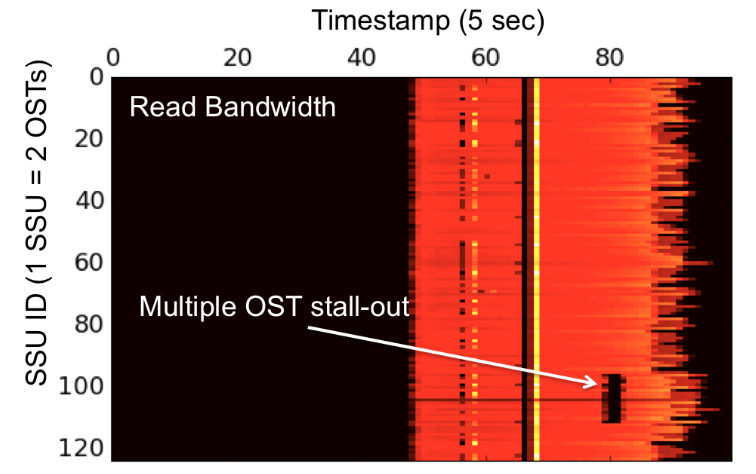
\includegraphics[width=0.8\columnwidth]{figs/example.png}
%\vspace{-.07in}
\caption{Example figure showing server-side read bandwidth with an artifact
caused by a Lustre server problem.}
\label{fig:example}
\vspace{-.1in}
\end{figure}

\begin{itemize}
\item Sometimes metadata operations are slow (e.g., file-per-process I/O)
    \begin{itemize}
    \item Show Darshan logs showing high metadata time
    \item Show LMT MDT logs showing high background metadata or CPU rate
    \item Show GPFS NSD metadata loads?  Can we do this?
    \end{itemize}
\item Sometimes hardware goes bad
    \begin{itemize}
    \item Show Darshan logs showing bad performance at the POSIX layer (i.e., not the
    application's fault)
    \item Show Lustre OSTs that stall out, e.g, Figure~\ref{fig:example}
    \item Show slow Lustre OSTs due to failover/oversubscription (a la Darshan 3 paper)
    \item Show poorly performing GPFS NSDs
    \end{itemize}
\item Sometimes there is interference from other applications
    \begin{itemize}
    \item Show Darshan logs showing bad performance at the POSIX layer (i.e., not the
    application's fault)
    \item Show jobs with and without background LMT load
    \item Show jobs with and without background mmpmon load
    \end{itemize}
\end{itemize}

\subsection{Discussion}

\begin{itemize}
\item Make statements about how often bad I/O performance can be attributed to each
of the different causes we categorized--that is, break down what the most
common sources of performance degradation are
\item Make statements about how susceptible different file systems are to these bad
I/O performance root causes to stir up controversy (GPFS is better/worse than
Lustre when facing problem X)
\item Propose that holistic I/O monitoring can provide a feedback loop for
coscheduling (to hit some buzzwords)
\end{itemize}

\section{Related work}

\todo{include SIOX, Xiaosong Ma's work}

\section{Conclusions}

\section{TEMPORARY: TECHNICAL TASKS}

Assumption: assignments here and in preceding text are tentative, and really
just guess at someone who can keep tabs on that activity.  Can re-assign,
delegate, pull in more people, etc.

Assumption: although the paper as outlined will focus on Cori and Mira, we
should actually try to do these things across Theta and Edison as well.  Four
total platforms, and we'll see which ones are most viable for study in paper.

To do:
\begin{itemize}
\item create git repository to store benchmarks, config files, job scripts,
and cron configs for our set of benchmarks \assign{Shane}
\item get new version of HACC-IO benchmark and parameters \assign{Suren}
\item get Boxlib benchmark and parameters \assign{Glenn}
\item gather standard VPIC parameters \assign{William}
\item gather standard IOR parameters \assign{Glenn}
\item make sure that mmpmon monitoring gets deployed on Mira \assign{Phil and
Kevin}
\item coordinate LMT monitoring methods on Theta \assign{Glenn and Kevin}
\item enable cron jobs to run periodic jobs on ALCF machines \assign{Shane}
\item enable cron jobs to run periodic jobs on NERSC machines \assign{Glenn}
\item create and enable cron jobs to check Lustre failover status
\assign{Glenn}
\item create and enable cron jobs to check Lustre server capacity
\assign{Glenn}
\item create and enable cron jobs to check GPFS failover status
\assign{Shane}
\item create and enable cron jobs to check GPFS server capacity
\assign{Shane}

\end{itemize}

Timeline:
\begin{itemize}
\item Start running periodic (daily) jobs by mid-January
\item writing up text based on results by mid-February
\end{itemize}

Stretch goals:
\begin{itemize}
\item additional instrumentation sources
\item more contributions from analysis framework perspective (i.e.,
leveraging work from William's paper) 
\item deploy on more platforms (either additional ALCF or NERSC systems, or
reach out to another facility like Blue Waters)
\end{itemize}

\bibliographystyle{IEEEtran}
\bibliography{REFERENCES}


\end{document}
